%! Author = Len Washington III
%! Date = 2/15/24

% Preamble
\documentclass[lab={2},title={Voice Onset Time}]{com310lab}

% Packages


% Document
\begin{document}

\maketitle

\begin{overview}
	Consonants of all stripes can be classified as to whether they are voiced or voiceless, but the exact cut to voicing varies across consonant types as well as across different languages.
	For example, stop consonants, regardless of voicing, generally show some degree of vocal fold vibration when they occur immediately before a vowel.
	Likewise, an acoustic cue that counts as voiced in one language many not count as voiced in another.\\

	A ``cue'' is a physical property of the speech that helps a listener correctly recognize a speech sound.
	For example, one cue to voicing for stop consonants is called ``voice onset time,'' or VOT, which refers to the time interval between when the articulators release after a closure and when voicing begins.
	Consider the VOT for a typical voiceless alveolar stop in American English, such as the \ipa{/t/} in `top':
	the tongue tip makes contact with alveolar ridge and makes a complete seal for a period of time.
	This period of closure is seen in a waveform as a period of silence and no detectable waves.
	Then, there is a release of the tongue tip, which can be seen as a sudden brief burst of acoustic energy (intense aperiodic waves).
	Following this, there is an interval of time when there is no voicing, but there is a period of low-frequency turbulence associated with aspiration.
	Lastly, voicing for the vowel begins.
	This can be seen in a waveform when near-identical waves set up at regular intervals--around 1 wave every 10 milliseconds or so (1 second = 1000 milliseconds).\\

	VOT is measured from the moment of release to the moment voicing begins.
	It is reported in milliseconds.
	Figure~\ref{fig:vot} below shows different measurements of VOT\@.
	It can be a positive value when the release occurs before voicing begins (right waveform),
	it can be a negative value when voicing precedes the release (left waveform), and VOT is 0 when the release and voice occur simultaneously (middle waveform).

	\begin{figure}[H]
		\centering
		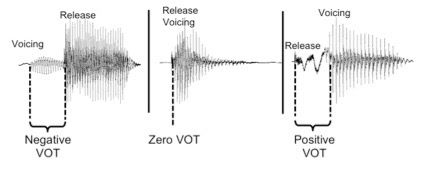
\includegraphics[width=\textwidth]{vot}
		\caption{Three different VOT values based on the onset of voicing relative to the release of active articulators.}
		\label{fig:vot}
	\end{figure}~
\end{overview}

\begin{problem}
	English makes a two-way distinction among stop consonants at each place of articulation: each is either voiced or voiceless.
	Thai makes a three-way distinction: stops are voiced, voiceless or voiceless aspirated.
	Hindi makes a four-way distinction among stops: they are voiced, voiceless, voiceless aspirated, or voiced aspirated.
	(Examples for the alveolar/dental and labial series for each language are given below.)
	However, it is unclear what physical property helps listeners distinguish among the different sounds.
	At issue is whether VOT is a reliable physical indicator of the different kinds of stop consonants and whether there is variation in VOT across the three languages.

	\begin{table}[H]
		\centering
		\label{tab:languages}
		\begin{tabular}{p{0.3\textwidth} *{5}{ p{0.08\textwidth} } p{0.15\textwidth}}
			& \multicolumn{2}{p{0.2\textwidth}}{\textbf{English}} & \multicolumn{2}{p{0.2\textwidth}}{\textbf{Thai}} & \multicolumn{2}{p{0.2\textwidth}}{\textbf{Hindi}}\\
			\textbf{Labial-series} & & & & & & \\
			voiced & \ipa{/ber/} & `bear' & \ipa{/ba/} & `crazy' & \ipa{/bal/} & `hair'\\
			voiceless aspirated & \ipa{/per/} & `pear' & \ipa{/p\super h{}a/} & `cloth' & \ipa{/p\super h{}a/} & `knife-blade'\\
			voiceless unaspirated & & & \ipa{/pa/} & `aunt' & \ipa{/pa/} & `take care of'\\
			voiced aspirated & & & & & \ipa{/b\super h{}al/} & `forehead'\\
			\textbf{Alveolar/dental-series} & & & & & & \\
			voiced & \ipa{/der/} & `dare' & \ipa{/da:/} & `curse' & \ipa{/dal/} & `lentil'\\
			voiceless aspirated & \ipa{/ter/} & `tear' & \ipa{/t\super h{}a:/} & `landing' & \ipa{/t\super h{}a/} & `plate'\\
			voiceless unaspirated & & & \ipa{/ta:/} & `eye' & \ipa{/tal/} & `beat'\\
			voiced aspirated & & & & & \ipa{/d\super h{}al/} & `knife'\\
		\end{tabular}
	\end{table}~
\end{problem}

\begin{task}
	Retrieve files containing stop consonants for English, Thai, and Hindi, using Praat and the guide above, measure VOT for all files.
	The files will be made available in a flash drive, and they will also be made available on a shared Google Drive file (check your email for an invitation to view the file folder).
	The file names correspond to the transcription and glosses (translations) above.
	A demonstration of how to measure VOT will be given at the beginning of the lab.\\

	Then, address the issue raised above: how does VOT distinguish among the various stop consonants with respect to voicing, and the extent you can, aspiration.
	Describe any variation in VOT across the three languages.
	Supply summary statistics and figures as needed.
	Report results for each language individually.
	Also, within each language, report results separately for the alveolar/dental stops and the labial stops.
\end{task}

\begin{writeup}
	Follow the format for writing up phonetics lab reports and upload your report on Blackboard.
\end{writeup}

\pagebreak

\labtitle

\begin{topic}
	\\
\end{topic}

\begin{issue}
	\\
\end{issue}

\begin{hypothesis}
	\\
\end{hypothesis}

\begin{method}
	\\
\end{method}

\begin{results}
	\\
\end{results}

\begin{discussion}
	\\
\end{discussion}

\end{document}